%% -1	\part{part}
%% 0	\chapter{chapter}
%% 1	\section{section}
%% 2	\subsection{subsection}
%% 3	\subsubsection{subsubsection}
%% 4	\paragraph{paragraph}
%% 5	\subparagraph{subparagraph}
%% \part and \chapter are only available in report and book document classes

\chapter{Introduction}
Here is presented the current landscape about the main topics of this thesis such as, how to measure heart rate, exams digitalization and standards, what is cloud computing and how does it apply to health activities.
\section{Cloud Computing}
\subsection{Definition}
Because a great number of interpretation and its flexibility, define precisely Cloud Computing is not an easy task. Both in literature and common speaking Cloud Computing has become a buzzword, even if it carries a concept already available 13 years ago which is Grid Computing and distributed systems in general \cite{foster}.\\
The largest part of computer scientists agree on defining cloud computing as\\
\textit{A large-scale distributed computing paradigm that is driven by economies of scale, in which a pool of abstracted, virtualized, dynamically-scalable, managed computing power, storage, platforms, and services are delivered on demand to external customers over the Internet.}\cite{foster}\\
Concluding, this paradigm with respect to the traditional ones, it is:
\begin{itemize}
    \item Massively scalable
    \item Delivers different levels of services to customers outside the cloud
    \item Dynamically scaled and over configuration
\end{itemize}

\subsection{Service models}
Here are presented the typical ways in which cloud services are made available to customers, these service models are often interdependent and synergetic each other, for example in figure \ref{fig:saas_paas_iaas} it is easy to see that PaaS is dependent in IaaS since applications platforms require a physical infrastructure.\\ \\
From an economic point of view this technology is particularly attractive for smaller companies and start-up, which want to avoid large up-front IT infrastructure investments \cite{CloudComputingModels}.\\
The figure \ref{fig:saas_paas_iaas} highlights customer with respect to provider roles among different service models.

\paragraph{Saas (Software as a Service)}
\label{paragraph:Saas}
This is the first proposed structure since the load demanded to providers is the greatest one among all the available models.
Consequently it enables a very quick online solution letting complete control to providers and paying through an as-you-use model, sometimes even for free.\\
SaaS delivers a web acces software using a "one to many" model, there are many popular examples as Microsoft office 365, Google Apps, Dropbox and Slack. \cite{saas_examples}\\ \\
It is not well suited when a software needs the lowest possible processing time (as real-time ones need) or is bounded by regulation and legislation which do not permit outsourcing data hosting.
\paragraph{Paas (Platform as a Service)}
\label{paragraph:Paas}
Platform as a Service model provides a pre-build application platform to customers, in this case it is not necessary to spend time building underlying infrastructure. Advantages are a quick and easy web application development at a cheaper cost.\\
PaaS provider dynamically scales infrastructure resources depending on applications needs, they also offers an API and a Web-based UI to for platform management.\\ \\
It is not recommended to use this kind of model when the subsequent features are required:
\begin{itemize}
    \item High portability (from/to different providers)
    \item Proprietary approaches or softwares usage
    \item Custom application performance settings 
\end{itemize}
\cite{CloudComputingModels}\cite{cloud_computing_stack_saas_paas_iaas}\\
Examples of popular PaaS providers are Heroku and Google App Engine.
\paragraph{Iaas (Infrastructure as a Service)}
\label{paragraph:Iaas}
It is the most customizable service model offered, it allows customers to handle directly their infrastructure components such as server virtual machines, network, storage, etc..\\
While a IaaS customer is outsourcing servers softwares, data-center space and network equipment to his provider, he can focus on the organization of its resources as services and configure their scaling policies.\\
The most popular IaaS provider is Amazon Web Services.
\paragraph{Serverless}
\label{paragraph:Serverless}
Differently from previously defined models, serverless computing (sometimes referred to as FaaS: Function as a Service \cite{sls_wikipedia}) enables developer to implement server-side logic and execute it in a stateless container that are event-triggered.\\
It still keeps the advantage to run code without provisioning or managing servers, leaving completely the resource management to the provider.
Furthermore the code does not require to be specifically built for a framework or library \cite{martin_serverless}.
The most popular FaaS implementation is AWS Lambda

\begin{figure}[h]
    \centering
    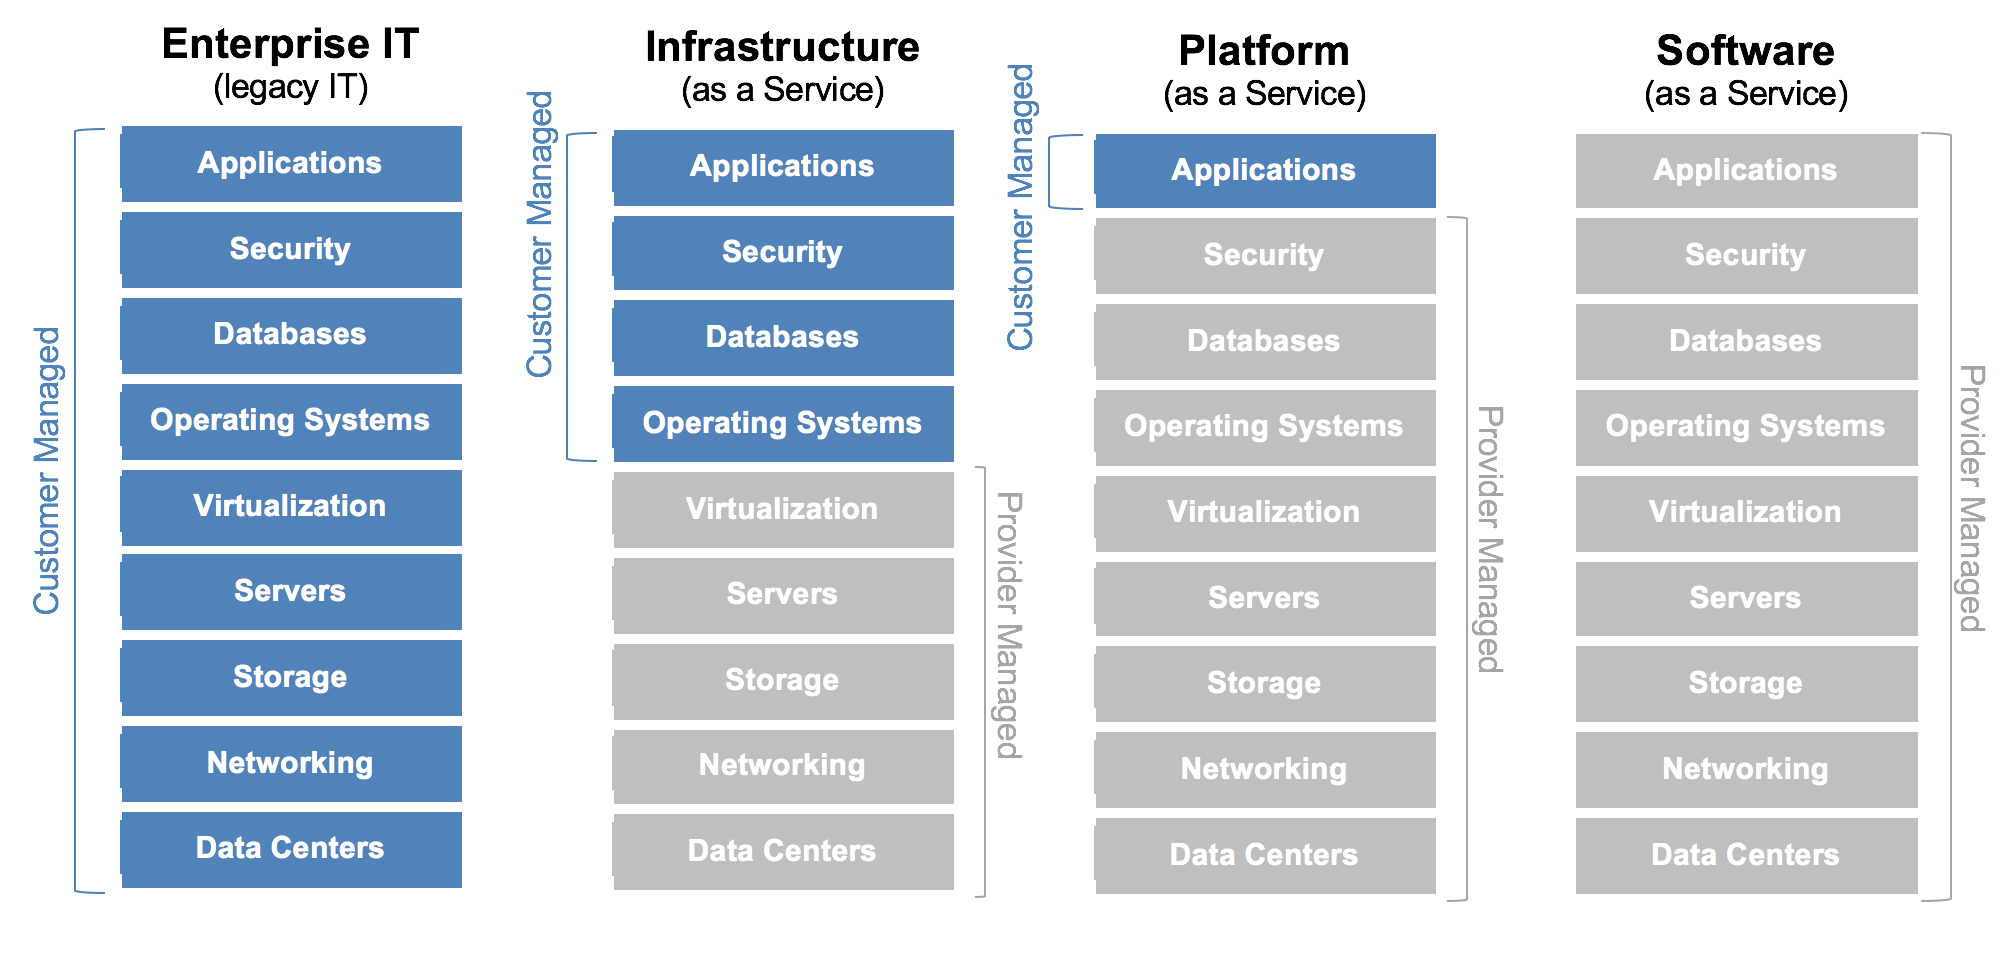
\includegraphics[width=\textwidth,keepaspectratio]{img/saas_paas_iaas}
    \caption{Comparing legacy IT service model with respect to SaaS,PaaS,IaaS}
    \label{fig:saas_paas_iaas}
\end{figure}

\subsection{Deployment models}

\paragraph{Private Cloud}
Service models described above con be deployed in different ways. The National Institute of Standard and Technology defines three main type of deployment: Private Cloud, Public Cloud and Hybrid Cloud. \cite{nist}
The main differences among them is who is granted to use a specific cloud infrastructure.
\label{paragraph:Private Cloud}
This kind of deployment enables just a single organization and its business units to use cloud resources.
Usually enabled stakeholders are directly the owner, a third party or a combination of them.
\paragraph{Public Cloud}
\label{paragraph:Public Cloud}
In this case everyone with an internet connection is allowed to use cloud resources. Public cloud are usually owned and managed by business, government and academic or a combination of them.
\paragraph{Hybrid Cloud}
\label{paragraph:Hybrid Cloud}
It is the combination of \textit{Private Cloud} and \textit{Public Cloud} which means that twi different deployments con be bounded together by standardized or proprietary technology.


\section{Web Services}
The aim of this thesis is also to show, how has been possible to make different systems speak each other.
It is impossible to understand this concept without a brief introduction to what webservices are.\\
\textit{"These are standardized way of integrating web-based applications using XML, SOAP, WSDL and UDDI open standards over an internet protocol backbone."}\cite{webservice}
Every web service offers a particular function at a defined network address where it is always available.\\
The main approaches to implement web services are two: the first one follows the REpresentational State Transfert (REST) principles where everything is built around the concept of resource, the last one is the Simple Object Access Protocol (SOAP) where particular emphasis is given to the service idea.\\
Follow a more detailed explanation.
\subsection{REST}
\label{subsection:REST}
A REST web service enable operations on several resources based on the type of request it receives.
With respect to SOAP it is directly based on HTTP protocol and is stateless: every forwarded request does not make the server save in any way the client state.\\
It is possible to get different responses from a REST webservice: from HTML web pages to JSON or XML formatted data, the only constraint is that web service has to support the data-type we are asking for.
Five principles sum up REST as web service development system:
\begin{itemize}
    \item Resource identification: dealing with web resources it is natural to identify them with URIs.
    \item HTTP methods usage: since HTTP is already well defined, CRUD operations have been mapped to the protocol verbs.
    \item Self descriptive messages: Data format of the representation which is sent to the client, must always come with its media type.
    \item HATEOAS - Hypermedia As The Engine Of Application State: resources should be  each other through hypertext.
    \item Stateless: because HTTP protocol is stateless too, the client state is never managed by servers.
\end{itemize}
In particular HTTP protocol verbs have been mapped in this way:
\begin{itemize}
    \item GET mapped as Read
    \item POST mapped as Create
    \item PUT mapped as Update
    \item DELETE mapped as Delete
\end{itemize}
\subsection{Soap}
\label{subsection:Soap}
Despite REST principles, Soap is a well defined protocol and it is not bounded to HTTP. It implements a way to exchange messages over different applications where the transport protocol can be anyone.\\
SOAP enables the usage of Web Service Description Language (WSDL) in order to define the API and eventually allow the automatic generation of client libraries.
Although the aim is the same of REST, this kind of approach is explicitly different because it builds a web independent infrastructure.

\section{Standard for Interoperability}
\subsection{12-lead ECG}
\label{subsection:12leadecg}
12-Lead Ecg is one of the most used methodology in clinical cardiac medicine, it is performed by attaching 10 electrodes on the surface of the limbs and the chest and then 12 groups of signals are generated while their signal recorded. The overall magnitude of the heart's electrical potential is then measured from twelve different angles (called leads) and is recorded in seconds over a period of time.\\
The graph of voltage versus time is referred to as electrocardiogram, which is considered the main tool for standard ECG analysis. \cite{electrocardiography_it} \cite{electrocardiography_en}\\
This methodology is fundamental for Myocardial infarction, Ischemia, Heart arrhythmia, Heart failure, Artificial cardiac pacemaker interested patients. Traditionally each instrument generates vendor-specific waveform data formats which are compressed or encrypted by their own algorithms.\\
Instruments used for clinical 12-lead ECG recording are bounded to the use in hospital or clinics. Still 12-lead ECG reports are unavailable in remote or difficult to reach areas, especially for emergency cases where speed is essential. Indeed different 12-lead ECG instruments and specialists interpretation skills are barriers against a reliable healthcare.
\cite{Hsieh2012}

\subsection{ECG Digitalization}
\label{subsection:ecgdigitaliation}
The increasing spread of IT technologies over healthcare systems, made the management of digital electrocardiogram signals one of the most debated and investigated topic in e-health literature. Because an uncoordinated development of several standard the convergence to a unique format has been a key issue. \cite{trigo} The current landscape is a wide variety of different file format and standard which surely makes the creation of end to end and standardized solution more challenging, even if lots of mapping procedures over ECG formats has been created as open source softwares.\\
Although the standards situation makes development more difficult, there are many examples in literature using a common SCP-ECG file format to store cardiac wave forms, some of them are reported in \cite{trigo}. This is a clear signal of a general interest around SCP-ECG as a standard by the scientific community. The history of the standard starts in 1989-1990 when European, American and Japanese manufacturers jointly worked and agreed on SCP-ECG development, to allow full interoperability between ECG devices and generic host systems.\\
The aim was to exchange ECG signals and related metadata.
Later in 1993 it became an European ENV code (Europäische Norm Vorübergehend: a provisional eurocode to indicate a test period), but became an offical EN eurocode only in 2005, after two years in 2007 it has been revised and later in 2009 adopted as an ISO (ISO 11073-91064:2009).\\
In 2014 a team which mission was to maintain and update SCP-ECG standard. Their tasks comprehended remove, revision and extend the file format parts taking into account new methodologies and technologies.\cite{danilopani}\\
The standard addresses specifically compression and communication of resting ECGs for different methodologies such as Holter, Exercise ECGs and real-time monitoring.\\
In 2002, the first open source online platform for SCP-ECG certification and conformance testing has been developed.\cite{Chronaki}\\

\subsection{Electronical Health Record}
\label{subsection:electronic_health_record}
Medical record, medical chart and health record are different terms to describe the documentation of a patient history and care.\\
Traditionally, health records were written on paper, maintained in folders divided into sections based on the type of note, and only one copy was available.
Computer Technology developed in the 60s and 70s laid the foundation for the development of the Electronic Health Record.\\
As inadequacies of the paper record became increasingly more apparent in 1992, the American Institute of Medicine advocated a shift from a paper-based to an electronic medical record one.\cite{Evans2016ElectronicHR}\\
An Electronic Health Record (EHR) is defined as \textit{"a repository of many Electronic Medical Records (EMR), which are a digital version of a chart with patient information stored in a computer, it refers to everything possible to find in a paper chart, such as medical history, diagnoses, medications, immunization dates and allergies.}\cite{emr}\\
Indeed represents a medical record within a single facility, such as a doctor's office or a clinic.\\
Around 1992 in US, EHRs were developed and used at a number of academic inpatient and outpatient medical facilities, but none contained all the information in the paper chart and most EHRs today are still a hybrid collection of computerized and paper data.
\cite{Evans2016ElectronicHR}\\
Because the regionalization of the Italian Healthcare System, there exists discrepancies among the different areas of the country, which the use of IT technologies may be useful to solve. In 2010 the Italian government introduced the electronic health record (EHR) implementation, which includes a minimum core of essential documents that should be created and updated by general practitioners.\\
During March 2017 the Italian e-health experts met for an \textit{InnovationLab}, there were government agencies, CEO and managers of important health companies, national care administrators and scholars. Their aim was to unlock the Italian health welfare because the state inadequacy, completing rapidly the e-health plan and the EHR (aka Fascicolo Sanitario Elettronico). They ended up with the \textit{"Carta di Salerno"}: an agreement to project the Italian Smart Health.
In 2002, an experts group from Cup2000 Spa designed a regional e-health network called SOLE (Sanità OnLinE) which would be part of the FSE. Later in 2009 it was finally possible to the Regional Healthcare Users to use the system while in 2013 it became national law inside the \textit{"Digital Agenda"} proceedings.\\
Recently in 2015 the FSE has been technically defined and each region started its own repository with the related IT company.
\cite{smarthealth}\\
Even if it not clear when third-party stakeholders and companies which produces EMR will be able to submit their data to local repositories, it is known that such services will be available, at least for hospitals, through SOAP web services.

\subsection{Accredited organization}
To develop international healthcare interoperability standards a no-profit organization has been composed from several countries all over the world, Health Level 7 (HL7) \textit{is an international community of healthcare subject matter experts and information scientists collaborating to create a framework for the exchange, integration, sharing, and retrieval of electronic health information.} Its target is to spread the use and knowledge of open standard in healthcare informatic systems, to improve interoperability among different systems and their communication efficiency. \cite{health_level_seven}


\subsection{eHealth (Cloud Computing Application To Medical Device)}
E-Health underlies cloud computing for clinical use, which John Mitchell from Sydney university defines as:"\textit{The health industry's equivalent of e-commerce}". From an integration perspective, e-health are:"\textit{integrated healthcare systems}" whose sum is much more than the one obtained from the single components. Even if the meaning varies among different contexts \cite{Eysenbach} it is possible to define e-health as the set of technological themes in health today, whose initiatives do not originate necessarily with the patient. \cite{oh}\cite{DellaMea}
A technological improvement is represented by the e-health cloud computing birth, according to Foster et al. cloud computing is \textit{"A computing paradigm which is a pool of abstracted, virtualized, dynamically scalable, managing, computing power storage platforms and services  for on demand delivery over the Internet"} \cite{foster}, moreover cloud computing offers a pay-as-you-use model helping healthcare industry cope with current and future demands, keeping the cost minimum. \cite{AbuKhousa}
Already in 2012 was possible to observe many healthcare providers shifting the burden of managing and mantaining complex health information technologies (HIT) to the Cloud Service Providers. \cite{foster}
Infact the adoption of cloud computing technologies can significantly reduce IT costs while improving patient care services, solve resources scarcity problems due to distance and experts availability. \cite{AbuKhousa}
It is possible to find many examples of e-health cloud implementation, here are quoted some of the latest,\\\\
Shah J.Miah et al. developed an e-health consultancy system using cloud computing that enables doctors and healthcare workers to identify and treat non-communicable diseases in rural and remote communities in Bangladesh, a developing nation. \cite{MIAH2017311}\\\\
Sri Vijay BharatPeddi et al. propose a system able to classify food object inside a dish by a picture taken from a camera, then it is able to compute the overall calories intake with considerable accuracy. They said that \textit{"The novelty of the system is to avoid the  heavy offload of computational system functions to the cloud, but also employing an intelligent cloud-broker mechanism to strategically and efficiently utilize cloud instances"} \cite{PEDDI201771}\\\\
Mohamed Estai et al. showed a store-and-forward telemedicine platform “Remote-I” to assist in the screening of oral diseases using an image acquisition Android app operated by 17 teledental assistants. A total of 485 images (five images per case) were directly transmitted from the Android app to the server. Then a panel of five dental practitioners assessed the images and reported their diagnosis.\cite{mohamedestai}\\ \\
Still the resulting view of developed cloud systems for e-health documented in literature does not shows cardiac digital system similar to the Cardioline one. The reported examples are significantly smaller and simpler. Mostly they involve a lower number of stakeholders focusing just on providing an health service and not on the management part. In the discussed case it has been taken care both to the logic of the system administration: managing several tanants divided by units, users and patients and to the actual health service we aim to provide.